\documentclass[]{article}
\usepackage{lmodern}
\usepackage{amssymb,amsmath}
\usepackage{ifxetex,ifluatex}
\usepackage{fixltx2e} % provides \textsubscript
\ifnum 0\ifxetex 1\fi\ifluatex 1\fi=0 % if pdftex
  \usepackage[T1]{fontenc}
  \usepackage[utf8]{inputenc}
\else % if luatex or xelatex
  \ifxetex
    \usepackage{mathspec}
    \usepackage{xltxtra,xunicode}
  \else
    \usepackage{fontspec}
  \fi
  \defaultfontfeatures{Mapping=tex-text,Scale=MatchLowercase}
  \newcommand{\euro}{€}
\fi
% use upquote if available, for straight quotes in verbatim environments
\IfFileExists{upquote.sty}{\usepackage{upquote}}{}
% use microtype if available
\IfFileExists{microtype.sty}{%
\usepackage{microtype}
\UseMicrotypeSet[protrusion]{basicmath} % disable protrusion for tt fonts
}{}
\usepackage[margin=1in]{geometry}
\usepackage{color}
\usepackage{fancyvrb}
\newcommand{\VerbBar}{|}
\newcommand{\VERB}{\Verb[commandchars=\\\{\}]}
\DefineVerbatimEnvironment{Highlighting}{Verbatim}{commandchars=\\\{\}}
% Add ',fontsize=\small' for more characters per line
\usepackage{framed}
\definecolor{shadecolor}{RGB}{248,248,248}
\newenvironment{Shaded}{\begin{snugshade}}{\end{snugshade}}
\newcommand{\KeywordTok}[1]{\textcolor[rgb]{0.13,0.29,0.53}{\textbf{{#1}}}}
\newcommand{\DataTypeTok}[1]{\textcolor[rgb]{0.13,0.29,0.53}{{#1}}}
\newcommand{\DecValTok}[1]{\textcolor[rgb]{0.00,0.00,0.81}{{#1}}}
\newcommand{\BaseNTok}[1]{\textcolor[rgb]{0.00,0.00,0.81}{{#1}}}
\newcommand{\FloatTok}[1]{\textcolor[rgb]{0.00,0.00,0.81}{{#1}}}
\newcommand{\CharTok}[1]{\textcolor[rgb]{0.31,0.60,0.02}{{#1}}}
\newcommand{\StringTok}[1]{\textcolor[rgb]{0.31,0.60,0.02}{{#1}}}
\newcommand{\CommentTok}[1]{\textcolor[rgb]{0.56,0.35,0.01}{\textit{{#1}}}}
\newcommand{\OtherTok}[1]{\textcolor[rgb]{0.56,0.35,0.01}{{#1}}}
\newcommand{\AlertTok}[1]{\textcolor[rgb]{0.94,0.16,0.16}{{#1}}}
\newcommand{\FunctionTok}[1]{\textcolor[rgb]{0.00,0.00,0.00}{{#1}}}
\newcommand{\RegionMarkerTok}[1]{{#1}}
\newcommand{\ErrorTok}[1]{\textbf{{#1}}}
\newcommand{\NormalTok}[1]{{#1}}
\usepackage{graphicx}
\makeatletter
\def\maxwidth{\ifdim\Gin@nat@width>\linewidth\linewidth\else\Gin@nat@width\fi}
\def\maxheight{\ifdim\Gin@nat@height>\textheight\textheight\else\Gin@nat@height\fi}
\makeatother
% Scale images if necessary, so that they will not overflow the page
% margins by default, and it is still possible to overwrite the defaults
% using explicit options in \includegraphics[width, height, ...]{}
\setkeys{Gin}{width=\maxwidth,height=\maxheight,keepaspectratio}
\ifxetex
  \usepackage[setpagesize=false, % page size defined by xetex
              unicode=false, % unicode breaks when used with xetex
              xetex]{hyperref}
\else
  \usepackage[unicode=true]{hyperref}
\fi
\hypersetup{breaklinks=true,
            bookmarks=true,
            pdfauthor={Valentin Marquart},
            pdftitle={Übung 2},
            colorlinks=true,
            citecolor=blue,
            urlcolor=blue,
            linkcolor=magenta,
            pdfborder={0 0 0}}
\urlstyle{same}  % don't use monospace font for urls
\setlength{\parindent}{0pt}
\setlength{\parskip}{6pt plus 2pt minus 1pt}
\setlength{\emergencystretch}{3em}  % prevent overfull lines
\setcounter{secnumdepth}{0}

%%% Use protect on footnotes to avoid problems with footnotes in titles
\let\rmarkdownfootnote\footnote%
\def\footnote{\protect\rmarkdownfootnote}

%%% Change title format to be more compact
\usepackage{titling}

% Create subtitle command for use in maketitle
\newcommand{\subtitle}[1]{
  \posttitle{
    \begin{center}\large#1\end{center}
    }
}

\setlength{\droptitle}{-2em}
  \title{Übung 2}
  \pretitle{\vspace{\droptitle}\centering\huge}
  \posttitle{\par}
  \author{Valentin Marquart}
  \preauthor{\centering\large\emph}
  \postauthor{\par}
  \predate{\centering\large\emph}
  \postdate{\par}
  \date{2017-05-30}


\begin{document}

\maketitle


\begin{enumerate}
\def\labelenumi{\arabic{enumi}.}
\itemsep1pt\parskip0pt\parsep0pt
\item
  run io.R
\item
  import Data and do data wrangeling / clean up in external R.script
\item
  save cleaned data as RData file \texttt{cleandata.RData}
\item
  analyize and compute data here in RMD-chunks
\end{enumerate}

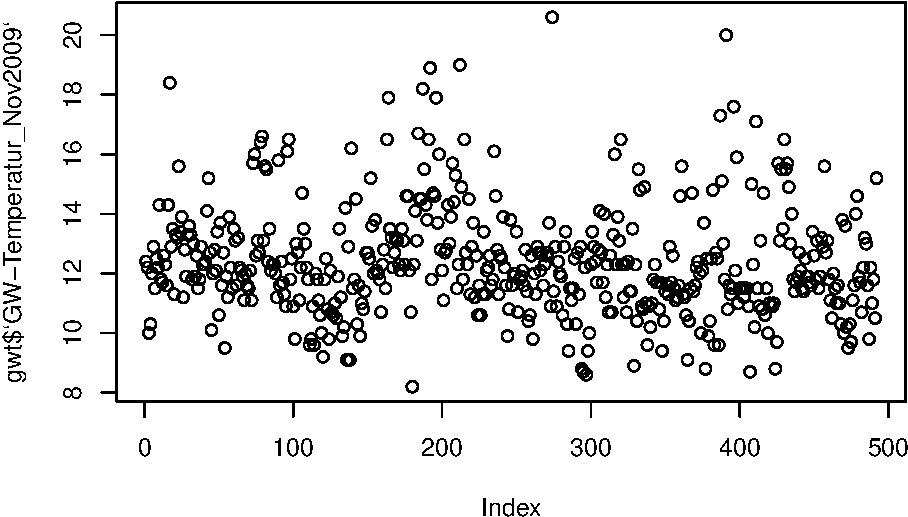
\includegraphics{Markdown-template_files/figure-latex/unnamed-chunk-1-1.pdf}

\begin{verbatim}
##     Min.  1st Qu.   Median     Mean  3rd Qu.     Max. 
##     0.00     0.01    18.43   525.30   317.40 10250.00
\end{verbatim}

\begin{Shaded}
\begin{Highlighting}[]
\CommentTok{# Do cool stuff with your imported data}
\KeywordTok{plot}\NormalTok{(gwt$}\StringTok{`}\DataTypeTok{GW-Temperatur2010}\StringTok{`}\NormalTok{)}
\end{Highlighting}
\end{Shaded}

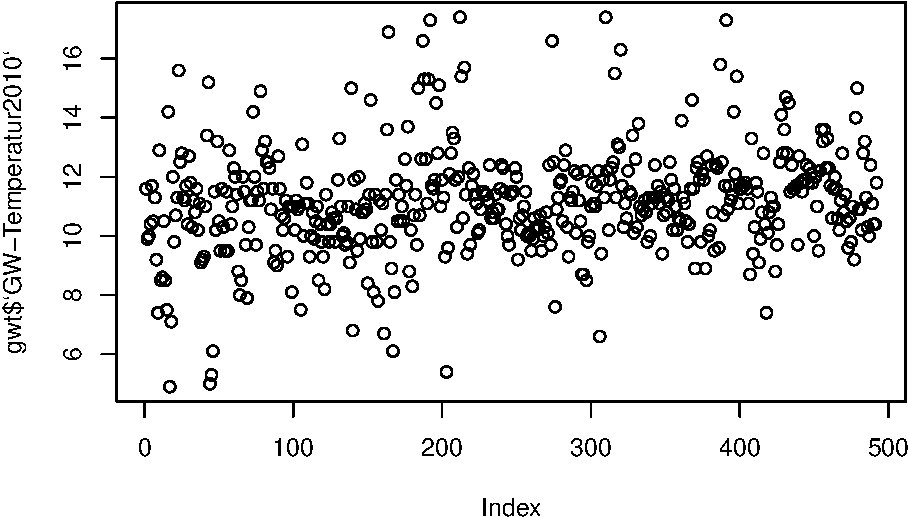
\includegraphics{Markdown-template_files/figure-latex/unnamed-chunk-2-1.pdf}

\newpage

\begin{Shaded}
\begin{Highlighting}[]
\NormalTok{n =}\StringTok{ }\DecValTok{100}
\NormalTok{p =}\StringTok{ }\FloatTok{0.03}
\NormalTok{x =}\StringTok{ }\KeywordTok{seq}\NormalTok{(}\DecValTok{0}\NormalTok{,}\DecValTok{30}\NormalTok{)}
\KeywordTok{par}\NormalTok{(}\DataTypeTok{mfrow=}\KeywordTok{c}\NormalTok{(}\DecValTok{1}\NormalTok{,}\DecValTok{3}\NormalTok{)) }\CommentTok{# Plot 3 figures, side by side}

\NormalTok{lambda_003 =}\StringTok{ }\NormalTok{n*p}
\NormalTok{p_x =}\StringTok{ }\NormalTok{(lambda_003^(x)/}\KeywordTok{factorial}\NormalTok{(x))*}\KeywordTok{exp}\NormalTok{(lambda_003)}
\KeywordTok{plot}\NormalTok{(p_x, }\DataTypeTok{type=}\StringTok{'b'}\NormalTok{,}\DataTypeTok{ylab=}\StringTok{'Poisson-Wahrscheinlichkeit p_x'}\NormalTok{,}\DataTypeTok{main=}\StringTok{'Poisson-Verteilung }\CharTok{\textbackslash{}n}\StringTok{ mit p=0.03'}\NormalTok{)}

\NormalTok{lambda_001 =}\StringTok{ }\NormalTok{n*}\FloatTok{0.01}
\NormalTok{p_x =}\StringTok{ }\NormalTok{(lambda_001^(x)/}\KeywordTok{factorial}\NormalTok{(x))*}\KeywordTok{exp}\NormalTok{(lambda_001)}
\KeywordTok{plot}\NormalTok{(p_x, }\DataTypeTok{type=}\StringTok{'b'}\NormalTok{,}\DataTypeTok{ylab=}\StringTok{'Poisson-Wahrscheinlichkeit p_x'}\NormalTok{, }\DataTypeTok{main=}\StringTok{'Poisson-Verteilung }\CharTok{\textbackslash{}n}\StringTok{ mit p=0.01'}\NormalTok{)}

\NormalTok{lambda_010 =}\StringTok{ }\NormalTok{n*}\FloatTok{0.1}
\NormalTok{p_x =}\StringTok{ }\NormalTok{(lambda_010^(x)/}\KeywordTok{factorial}\NormalTok{(x))*}\KeywordTok{exp}\NormalTok{(lambda_010)}
\KeywordTok{plot}\NormalTok{(p_x, }\DataTypeTok{type=}\StringTok{'b'}\NormalTok{,}\DataTypeTok{ylab=}\StringTok{'Poisson-Wahrscheinlichkeit p_x'}\NormalTok{,}\DataTypeTok{main=}\StringTok{'Poisson-Verteilung }\CharTok{\textbackslash{}n}\StringTok{ mit p=0.10'}\NormalTok{)}
\end{Highlighting}
\end{Shaded}

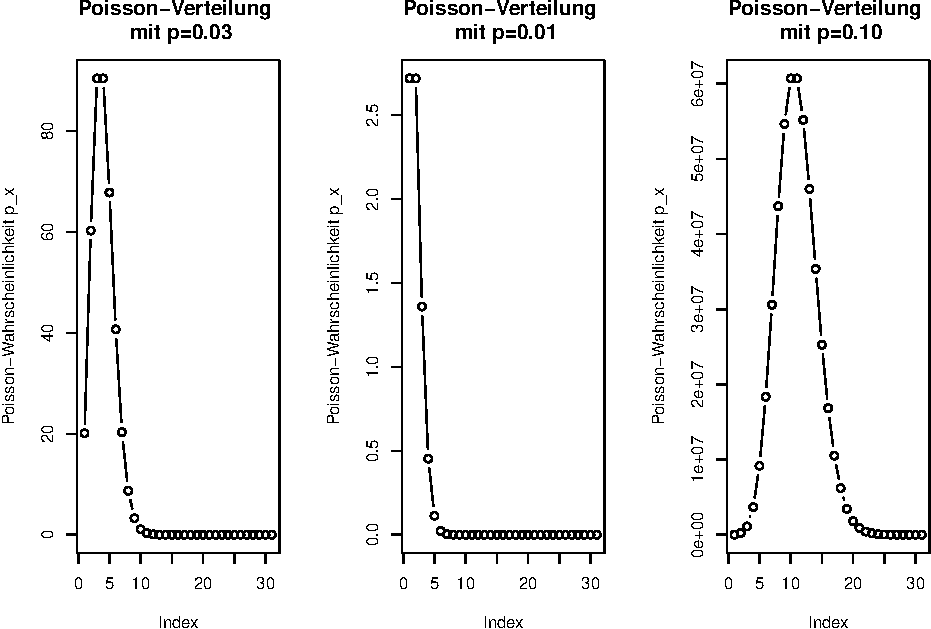
\includegraphics{Markdown-template_files/figure-latex/unnamed-chunk-3-1.pdf}

\newpage
Anmerkungen und Shortcuts ---

\itemize
\item Check Spelling \texttt{F7} \item Replace and Find
\texttt{Command+Shift+J} \item Compile PDF/HTML with
\texttt{CMD-SHIFT-K}

\end{document}
